\scanpage{49}
\mspage{5)}
% archive sheet number: 48
Cette opération de somme est la plus triviale parmi les opérations qu'il nous faudra expliciter et transcrire (combinatoirement) dans la suite. Notons de suite, pour $(X,\widetilde\Sigma,R)\deleted{\unsure{,}}$ donné
\[
X\deleted{\unsure{est}}\text{ connexe}\Longleftrightarrow\Gamma\mathrm{MD}(X,\widetilde\Sigma,R)\text{ connexe}
\]
plus précisément
\[
\pi_0(X)\simeq\pi_0(\Gamma\mathrm{MD}(X,\widetilde\Sigma,R))
\]
% slanted
\margin{\unsure{donner} la formule pour le genre d'un $\alpha\in\pi_0(X)\simeq\pi_0(\Gamma)$ en termes de la pondération -- plus généralement le \uline{genre total} est donné par $g=\sum_{s\in S}g_s+c(\Gamma)$\par $c(\Gamma)$: indice de connexion du graphe $=\deleted{\unsure{\mathrm{rg}}}\unsure{\mathrm{rg}\,H^1(\Gamma)|\dim H^1(\Gamma)}$}

\uline{Cas particuliers.}

a) Cas de $S_*\mathscr{T}_{\mathrm{top}}^{\pm}\deleted{\unsure{S_*\mathscr T_{\mathrm{top}}}}$ -- ici $\Sigma=\varnothing$, $\widetilde\Sigma=\partial X$.

Cela correspond aux graphes MD \deleted{qui} où \inserted{toutes les arêtes sont libres, i.e.} tous les sommets sont isolés (sauf arêtes libres) \deleted{\unsure{et}}\inserted{Graphe} est donc déterminé par
\diagram{\begin{tikzcd}[ampersand replacement=\&]
{A\ (\simeq\vec A=\vec A^\sigma)}\arrow[r,"r"]\arrow[d]\&\mathbb N\\
S\arrow[r,"\unsure{\gamma|g}"]\&\mathbb N
\end{tikzcd}}

Le cas de $\mathscr T_{\mathrm{top}}^{\pm}$ correspond à \unsure{admettre} $\rho=0$, donc la situation est donnée par
\diagram{\begin{tikzcd}[ampersand replacement=\&]
{A=A_0}\arrow[d]\&\\
S\arrow[r,"\gamma"]\&\mathbb N.
\end{tikzcd}}
\figure{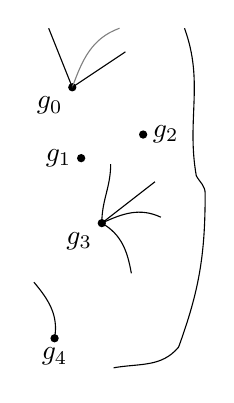
\begin{tikzpicture}[scale=.75]
\fill (0,3) circle (2pt);\node[below left] at (0,3){$g_0$};\draw (0,3)--(-.4,4);\draw[gray] (0,3) to[out=70,in=200] (.8,4);\draw (0,3)--(.9,3.6);
\fill (.15,1.8) circle (2pt);\node[left] at (.15,1.8){$g_1$};\fill (1.2,2.2) circle (2pt);\node[right] at (1.2,2.2){$g_2$};
\fill (.5,.7) circle (2pt);\node[below left] at (.5,.7){$g_3$};\draw (.5,.7) to[out=90,in=-90] (.65,1.7);\draw (.5,.7)--(1.4,1.4);\draw (.5,.7) to[out=25,in=155] (1.5,.8);\draw (.5,.7) to[out=-30,in=100] (1,-.15);
\fill (-.3,-1.25) circle (2pt);\node[below] at (-.3,-1.25){$g_4$};\draw (-.3,-1.25) to[out=80,in=-50] (-.65,-.3);
\draw (1.9,4) to[out=-70,in=100] (2.1,1.5) to[out=-60,in=90] (2.25,1.2) to[out=-90,in=70] (1.8,-1.4) to[out=-130,in=10] (.7,-1.75);
\end{tikzpicture}}

Le cas d'une structure connexe ($\mathrm{Card}.S=1$\inserted{i.e. $S=\{s\}$}) \deleted{type $(g,\nu)$ d'une structure} est \deleted{\unsure{déterminé par le genre}}\inserted{caractérisé} par la donnée des deux entiers $(g,\nu)$ ($g={}$genre, $\nu={}$nb de trous)
\[
g=\gamma(s),\quad\nu=\mathrm{card}\,A
\]
